\documentclass[11pt]{article}
\usepackage[margin=1in]{geometry}
\usepackage{amsmath,amssymb,amsthm}
% This TinyTeX install lacks grfext.sty, which epstopdf-base needs; all figures are PDF, so skip epstopdf.
\expandafter\def\csname ver@epstopdf-base.sty\endcsname{2020/01/24}
\usepackage{graphicx,booktabs,array}
\usepackage[round]{natbib}
\graphicspath{{../sims/out/}}
\setlength{\parindent}{0pt}\setlength{\parskip}{5pt}

\newtheorem{lemma}{Lemma}
\newtheorem{proposition}{Proposition}
\newtheorem{theorem}{Theorem}
\theoremstyle{remark}
\newtheorem*{remark}{Remark}

\title{SURE for the Single-Index Target:\\ Four Ways Around the Cross Term}
\author{Jack Wang}
\date{Working note, \today}

\begin{document}
\maketitle

\noindent
Section~4 showed that Stein's argument gets stuck for the single-index target. Steps~1 and~2 go through, but the cross term involves the ratio $f_{ij} = s_{0i}s_{0j}/s_{00}^2$, and its Stein expectations have no closed form. This note tries four other ways to estimate that one term. For each direction it plots the performance curve, that is, the estimated risk $\mathrm{SURE}(\alpha)$ against the true risk $R(\alpha)$ for $\alpha \in [0,1]$, with the minimizers $\hat\alpha$ and $\alpha^*$ marked. All four directions share every other piece of the SURE; they differ only in how they estimate the cross term.

\section{Assumptions}\label{sec:assumptions}

Every assumption used anywhere in the note is listed here. Each direction uses only some of them; Table~\ref{tab:assump} says which.

\begin{enumerate}
  \item[(A1)] \emph{Independent, identically distributed days.} The day-$t$ vectors $z_t = (m_t, x_t')'$ are i.i.d.\ over all days used: the $T$ current days and, for direction~\#5 and the pooled benchmarks of Section~\ref{sec:results}, the $T_0$ earlier days as well. (Theorem~\ref{thm:stale} itself needs i.i.d.\ only within the current window; see (A7).) This is what makes every sample moment an average of i.i.d.\ terms, so variances and covariances of sample moments are $1/T$ times daily ones. Realism: the standard working assumption, but daily returns show volatility clustering.
  \item[(A2)] \emph{Known zero mean.} $\mathbb{E}z_t = 0$. With this, $\mathbb{E}S = \Sigma$ holds with divisor $T$, which is the only condition of Yi's lemma. Realism: daily mean returns are tiny compared with their standard deviation, so this is close to true; with estimated means the divisors change.
  \item[(A3)] \emph{Observed market.} The market return $m_t$ is observed every day. It is a separate variable, not one of the $N$ assets, and $\sigma_m^2 = \operatorname{Var}(m_t) > 0$. This defines the target. Nothing in this note needs the market to be independent of the residuals or the single-index model to be true. Realism: good (an index return is observed). If the index contains the $N$ assets, nothing below changes, because $m_t$ simply enters $z_t$.
  \item[(A4)] \emph{Finite fourth moments.} $\mathbb{E}\|z_t\|^4 < \infty$. This makes $\operatorname{Var}(s_{ij})$ and $\operatorname{Cov}(m_t^2, x_{ti}x_{tj})$ finite, and it is what the distribution-free $\hat V$ of Section~5 needs. Realism: widely accepted for daily stock returns, though tails are heavy.
  \item[(A5)] \emph{Joint normality.} $z_t \sim N(0, J)$. This is needed only for the Stein identity behind direction~\#2. Realism: poor, since daily returns have excess kurtosis.
  \item[(A6)] \emph{Finite eighth moments.} $\mathbb{E}\|z_t\|^8 < \infty$. This is not needed for unbiasedness anywhere. It gives every SURE a finite variance, and it gives the $\sqrt T$ rates behind the large-$T$ approximations of \#3 and \#4. Realism: plausible for daily returns; it fails for $t$ tails with $\nu \le 8$.
  \item[(A7)] \emph{Independent earlier window.} Direction~\#5 uses betas $\tilde\beta$ computed from an earlier window of $T_0$ days that is independent of the current $T$ days, with $\mathbb{E}\tilde\beta_i^4 < \infty$ for every $i$. The fourth moment is needed because $\tilde R$ and $\tilde D$ involve second moments of $\tilde\beta_i\tilde\beta_j$; under normality, with $\tilde\beta_i = \tilde s_{0i}/\tilde s_{00}^2$, it holds when $T_0 > 4$. Under (A1), any disjoint earlier block of days qualifies. The unbiasedness of $\mathrm{SURE}_5$ needs only independence, not that the earlier window has the same distribution. Realism: the data exist in practice, but betas drift over time.
  \item[(A8)] \emph{Large $T$ (approximation regime).} Directions \#3 and \#4 replace an exact covariance by a first-order or resampling approximation whose error is of smaller order as $T \to \infty$ with $N$ fixed. This is not a condition for the formulas to be defined; it is the regime in which they are accurate. Realism: $T = 30$ is small and $T = 120$ is moderate.
\end{enumerate}

\begin{table}[h]
\centering
\caption{Which direction uses which assumption ($\checkmark$ = needed; (a) = needed only for the approximation to be accurate).}\label{tab:assump}
\begin{tabular}{@{}lcccccccc@{}}
\toprule
Direction & A1 & A2 & A3 & A4 & A5 & A6 & A7 & A8 \\
\midrule
Common pieces ($\hat V$, $\|F - S\|^2$) & $\checkmark$ & $\checkmark$ & $\checkmark$ & $\checkmark$ & & & & \\
\#2 plug-in Stein & $\checkmark$ & $\checkmark$ & $\checkmark$ & $\checkmark$ & $\checkmark$ & & & (a) \\
\#3 delta method (LW 2003) & $\checkmark$ & $\checkmark$ & $\checkmark$ & $\checkmark$ & & (a) & & (a) \\
\#4 bootstrap & $\checkmark$ & $\checkmark$ & $\checkmark$ & $\checkmark$ & & (a) & & (a) \\
\#5 stale $\beta$ & $\checkmark$ & $\checkmark$ & $\checkmark$ & $\checkmark$ & & & $\checkmark$ & \\
\bottomrule
\end{tabular}
\end{table}

For \#2, (A8) is marked because even under normality the plug-in step is only approximately unbiased.

\section{Setup and the risk decomposition}

\paragraph{Data and target.}
On day $t$ we observe the market return $m_t$ and the asset vector $x_t \in \mathbb{R}^N$, with $x_{ti}$ the return on asset $i$. Write $J = \operatorname{Cov}(z_t)$ for the $(N+1)\times(N+1)$ joint covariance, indexed from $0$ (the market) to $N$. So $J_{00} = \sigma_m^2$, $J_{0i} = \sigma_{0i} = \operatorname{Cov}(m_t, x_{ti})$, and $J_{ij} = \sigma_{ij}$ for $i,j \ge 1$; $\Sigma = (\sigma_{ij})$ is the asset covariance we want. The sample moments (known zero mean, divisor $T$) are
\[
  S = \frac{1}{T}\sum_{t=1}^T x_t x_t', \qquad
  s_{00}^2 = \frac{1}{T}\sum_{t=1}^T m_t^2, \qquad
  s_{0i} = \frac{1}{T}\sum_{t=1}^T m_t x_{ti}, \qquad
  \hat\beta_i = \frac{s_{0i}}{s_{00}^2}.
\]
The single-index target of \citet{ledoit2003}, following \citet{sharpe1963}, is $F = s_{00}^2\hat\beta\hat\beta' + \hat\Delta$, where $\hat\Delta$ is diagonal with the residual variances $\hat\delta_{ii} = \frac{1}{T}\sum_t (x_{ti} - \hat\beta_i m_t)^2$. Off the diagonal,
\[
  f_{ij} = s_{00}^2\hat\beta_i\hat\beta_j = \frac{s_{0i}s_{0j}}{s_{00}^2}, \qquad i \ne j.
\]

\begin{lemma}\label{lem:diag}
$f_{ii} = s_{ii}$ for every $i$. The target has the same diagonal as $S$, so shrinkage leaves the diagonal of $S$ unchanged.
\end{lemma}

\begin{proof}
Expanding the square, $\hat\delta_{ii} = s_{ii} - 2\hat\beta_i s_{0i} + \hat\beta_i^2 s_{00}^2 = s_{ii} - s_{0i}^2/s_{00}^2$, using $\hat\beta_i = s_{0i}/s_{00}^2$. Hence $f_{ii} = s_{00}^2\hat\beta_i^2 + \hat\delta_{ii} = s_{0i}^2/s_{00}^2 + s_{ii} - s_{0i}^2/s_{00}^2 = s_{ii}$.
\end{proof}

This uses the divisor $T$ in both $\hat\delta_{ii}$ and $s_{ii}$. With divisor $T-2$ in $\hat\delta_{ii}$, as in some regression software, the identity fails. Numerically, $\max_i|f_{ii} - s_{ii}| = 1.3\times10^{-15}$.

The estimator is $\hat\Sigma(\alpha) = \alpha F + (1-\alpha)S$ and the loss is $\|\hat\Sigma(\alpha) - \Sigma\|^2$ (squared Frobenius norm).

\paragraph{Risk decomposition.}
By (A1)--(A2), $\mathbb{E}S = \Sigma$, so Yi's lemma \citep{yi2013} applies. As in Section~5 (Lemma~\ref{lem:diag} does not change the algebra),
\[
  R(\alpha) = \alpha^2 D + (1 - 2\alpha)V + 2\alpha C, \qquad
  D = \mathbb{E}\|F - S\|^2,\quad V = \sum_{i,j}\operatorname{Var}(s_{ij}),\quad C = \sum_{i,j}\operatorname{Cov}(f_{ij}, s_{ij}).
\]
\emph{Diagonal bookkeeping.} By Lemma~\ref{lem:diag}, $\operatorname{Cov}(f_{ii}, s_{ii}) = \operatorname{Var}(s_{ii})$. Split $V = V_{\mathrm{diag}} + V_{\mathrm{off}}$ into its $i = j$ and $i \ne j$ parts, and write
\[
  C = V_{\mathrm{diag}} + C_{\mathrm{off}}, \qquad C_{\mathrm{off}} = \sum_{i \ne j}\operatorname{Cov}(f_{ij}, s_{ij}).
\]
Then $R(\alpha) = V_{\mathrm{diag}} + \alpha^2 D + (1 - 2\alpha)V_{\mathrm{off}} + 2\alpha C_{\mathrm{off}}$. The diagonal contributes the constant $V_{\mathrm{diag}}$, as it should, since the diagonal is never shrunk. Only off-diagonal entries enter $D$. The minimizer is
\[
  \alpha^* = \frac{V - C}{D} = \frac{V_{\mathrm{off}} - C_{\mathrm{off}}}{D}.
\]

\paragraph{What is computable.}
Two of the three unknowns are already solved.
\begin{itemize}
  \item $D$ is the mean of the observable $\|F - S\|^2$.
  \item $V$ is estimated without bias, under (A1), (A2) and (A4) only, by the distribution-free estimator of Section~5,
  \[
    \hat V = \frac{1}{T(T-1)}\sum_{t=1}^T\|x_tx_t' - S\|^2, \qquad
    \hat V_{\mathrm{diag}} = \frac{1}{T(T-1)}\sum_{t=1}^T\sum_{i=1}^N\left(x_{ti}^2 - s_{ii}\right)^2 .
  \]
\end{itemize}
Every direction below uses this $\hat V$ and $\|F - S\|^2$. A direction $d$ supplies an estimate $\hat C_{\mathrm{off}}^{(d)}$, and we set $\hat C^{(d)} = \hat V_{\mathrm{diag}} + \hat C_{\mathrm{off}}^{(d)}$ and
\[
  \mathrm{SURE}_d(\alpha) = \alpha^2\|F - S\|^2 + (1 - 2\alpha)\hat V + 2\alpha\hat C^{(d)}, \qquad
  \hat\alpha_d = \frac{\hat V - \hat C^{(d)}}{\|F - S\|^2} = \frac{\hat V_{\mathrm{off}} - \hat C_{\mathrm{off}}^{(d)}}{\|F - S\|^2},
\]
clipped to $[0,1]$. Since $\mathbb{E}\,\mathrm{SURE}_d(\alpha) - R(\alpha) = 2\alpha\,(\mathbb{E}\hat C_{\mathrm{off}}^{(d)} - C_{\mathrm{off}})$, the curve is unbiased at every $\alpha$ exactly when $\hat C_{\mathrm{off}}^{(d)}$ is unbiased. The ratio $\mathbb{E}\hat C^{(d)}_{\mathrm{off}}/C_{\mathrm{off}}$ is therefore the summary of each direction's bias.

\paragraph{Why $C$ is the hard term.}
For $\nu I$ the cross term was $\operatorname{Var}(\operatorname{tr}S)/N$, a variance of an average, which a sample variance estimates without bias. Here $f_{ij}$ is a ratio with the random $s_{00}^2$ in the denominator. Stein's lemma still turns $\operatorname{Cov}(f_{ij}, s_{ij})$ into expectations of derivatives, but those are expectations of ratios with no closed form in the population moments (Section~4.6). Nor is $f_{ij}$ an average of daily terms, so the Section~5 trick does not apply either. The four directions below are four ways around this.

\section{The four directions}

\subsection{Direction \#2: plug-in Stein}

\emph{Idea.} Run Stein's lemma on the joint vector $(m_t, x_t)$, which is exact under normality, and then replace the unknown covariances that it leaves behind by their sample versions.

\begin{lemma}[Joint Stein identity]\label{lem:joint-stein}
Assume (A1), (A2), (A5). For every smooth $h(z_1, \dots, z_T)$ with integrable derivatives, and $i, j \ge 1$,
\[
  \mathbb{E}\left[h\,(x_{ti}x_{tj} - \sigma_{ij})\right] = \sum_{k=0}^N J_{ik}\,\mathbb{E}\left[x_{tj}\,\frac{\partial h}{\partial z_{tk}}\right],
  \qquad
  \mathbb{E}\left[h\,(s_{ij} - \sigma_{ij})\right] = \frac{1}{T}\sum_{t=1}^T\sum_{k=0}^N J_{ik}\,\mathbb{E}\left[x_{tj}\,\frac{\partial h}{\partial z_{tk}}\right],
\]
where $z_{t0} = m_t$, $z_{tk} = x_{tk}$ for $k \ge 1$, and $J_{i0} = \sigma_{0i}$.
\end{lemma}

\begin{proof}
This mirrors the Stein covariance lemma of Section~4 with $z_t$ in place of $x_t$. Condition on the other days, so that $z_t \sim N(0, J)$. The multivariate Stein lemma for $z_t$ gives $\mathbb{E}[z_{ti}\varphi] = \sum_{k=0}^N J_{ik}\mathbb{E}[\partial\varphi/\partial z_{tk}]$. Take $\varphi = x_{tj}h$. Then $\partial\varphi/\partial z_{tk} = \delta_{jk}h + x_{tj}\,\partial h/\partial z_{tk}$, and the $\delta_{jk}$ term never fires for $k = 0$, because $j \ge 1$. So
\[
  \mathbb{E}[x_{ti}x_{tj}h] = \sigma_{ij}\mathbb{E}[h] + \sum_{k=0}^N J_{ik}\mathbb{E}[x_{tj}\,\partial h/\partial z_{tk}].
\]
Subtract $\sigma_{ij}\mathbb{E}h$ and average over $t$.
\end{proof}

\emph{Derivatives of $f_{ij}$.} Write $a_i = s_{0i}$ and $b = s_{00}^2$, so $f_{ij} = a_ia_j/b$. Since $\partial a_i/\partial x_{tk} = \delta_{ik}m_t/T$, $\partial a_i/\partial m_t = x_{ti}/T$, $\partial b/\partial m_t = 2m_t/T$ and $\partial b/\partial x_{tk} = 0$,
\[
  \frac{\partial f_{ij}}{\partial x_{tk}} = \frac{m_t(\delta_{ik}a_j + \delta_{jk}a_i)}{Tb}, \qquad
  \frac{\partial f_{ij}}{\partial m_t} = \frac{x_{ti}a_j + x_{tj}a_i}{Tb} - \frac{2m_t\,a_ia_j}{Tb^2}.
\]
Insert these into Lemma~\ref{lem:joint-stein} and sum over $t$, using $\sum_t x_{tj}m_t = Ta_j$, $\sum_t x_{tj}x_{ti} = Ts_{ij}$ and $\sum_t x_{tj}^2 = Ts_{jj}$. For $i \ne j$ this gives
\begin{equation}\label{eq:stein-exact}
  \operatorname{Cov}(f_{ij}, s_{ij}) = \frac{1}{T}\,\mathbb{E}\left[\frac{\sigma_{ii}a_j^2 + \sigma_{ij}a_ia_j + \sigma_{0i}(s_{ij}a_j + s_{jj}a_i)}{b} - \frac{2\sigma_{0i}\,a_ia_j^2}{b^2}\right].
\end{equation}
This is exact under normality. It is the expectation of a ratio, which is why Section~4 stopped here.

\emph{Integrability.} By Cauchy--Schwarz, $a_i^2 \le b\,s_{ii}$, so every term inside \eqref{eq:stein-exact} is bounded by a polynomial in the entries of $S$ times $b^{-1/2}$. Under normality, $b \sim \sigma_m^2\chi^2_T/T$ has $\mathbb{E}b^{-1} < \infty$ for $T > 2$, so Hölder's inequality gives integrability for $T \ge 3$.

\emph{Plug-in.} Replace $\sigma_{ii}, \sigma_{ij}, \sigma_{0i}$ by $s_{ii}, s_{ij}, a_i$ and drop the expectation. The result is symmetric in $(i,j)$:
\[
  \hat C_{\mathrm{off}}^{(2)} = \frac{1}{T}\sum_{i \ne j}\left[\frac{s_{ii}s_{0j}^2 + s_{jj}s_{0i}^2 + 2s_{ij}s_{0i}s_{0j}}{s_{00}^2} - 2f_{ij}^2\right].
\]

\emph{Exact or approximate?} Approximate, for two reasons. First, the plug-in is correlated with the bracket it multiplies: $\mathbb{E}[s_{ii}a_j^2/b] \ne \sigma_{ii}\mathbb{E}[a_j^2/b]$. The resulting bias is of relative order $1/T$, so the estimate is consistent but not unbiased. Second, \eqref{eq:stein-exact} itself needs (A5). For elliptical (Gaussian scale-mixture) data with positive excess kurtosis, such as the multivariate $t$, the fourth-moment terms are larger than the Gaussian formula says, and $\hat C^{(2)}$ underestimates the covariance. For other non-Gaussian laws the sign of the error is not determined.

\begin{remark}
Under normality, Isserlis' formula gives
\[
  \operatorname{Cov}(m_tx_{ti}, x_{ti}x_{tj}) = \sigma_{0i}\sigma_{ij} + \sigma_{0j}\sigma_{ii}, \qquad \operatorname{Cov}(m_t^2, x_{ti}x_{tj}) = 2\sigma_{0i}\sigma_{0j}.
\]
Substituting these into the delta-method formula of \#3 below, and then plugging in sample moments, gives exactly $\hat C^{(2)}_{\mathrm{off}}$. So plug-in Stein is the delta method with Gaussian fourth moments. It differs from \#3 only in how it estimates the fourth-moment terms.
\end{remark}

\emph{Cost.} $O(N^2)$ after $S$ and $s_{0\cdot}$.

\subsection{Direction \#3: the Ledoit--Wolf (2003) delta method}

\emph{Idea.} $f_{ij} = g(s_{0i}, s_{0j}, s_{00}^2)$ with $g(u,v,w) = uv/w$ is a smooth function of three sample means. Linearize $g$, and the covariance of $f_{ij}$ with $s_{ij}$ becomes a combination of covariances between sample means. Each of those is a daily covariance divided by $T$, which a sample covariance estimates. This is the device \citet{ledoit2003} use for their $\hat\rho$.

\emph{Formula.} The gradient of $g$ is $(v/w,\, u/w,\, -uv/w^2)$. To first order,
\[
  \operatorname{Cov}(f_{ij}, s_{ij}) \approx \frac{s_{0j}}{s_{00}^2}\operatorname{Cov}(s_{0i}, s_{ij}) + \frac{s_{0i}}{s_{00}^2}\operatorname{Cov}(s_{0j}, s_{ij}) - \frac{s_{0i}s_{0j}}{s_{00}^4}\operatorname{Cov}(s_{00}^2, s_{ij}).
\]
Strictly, the gradient is at the population point; we evaluate it at the sample point. Under (A1), each covariance of sample means is exact: $\operatorname{Cov}(s_{0i}, s_{ij}) = \operatorname{Cov}(m_tx_{ti}, x_{ti}x_{tj})/T$ and $\operatorname{Cov}(s_{00}^2, s_{ij}) = \operatorname{Cov}(m_t^2, x_{ti}x_{tj})/T$. With $\widehat{\operatorname{Cov}}(u,v) = \frac{1}{T-1}\sum_t(u_t - \bar u)(v_t - \bar v)$ the usual unbiased sample covariance of daily series, define
\[
  K_{ij} = \frac{1}{T}\widehat{\operatorname{Cov}}(m_tx_{ti},\, x_{ti}x_{tj}), \qquad
  L_{ij} = \frac{1}{T}\widehat{\operatorname{Cov}}(m_t^2,\, x_{ti}x_{tj}),
\]
\[
  \hat C_{\mathrm{off}}^{(3)} = \sum_{i \ne j}\left[\frac{s_{0j}}{s_{00}^2}K_{ij} + \frac{s_{0i}}{s_{00}^2}K_{ji} - \frac{s_{0i}s_{0j}}{s_{00}^4}L_{ij}\right].
\]
Note $K_{ji} = \widehat{\operatorname{Cov}}(m_tx_{tj}, x_{tj}x_{ti})/T$.

\emph{Exact or approximate?} Approximate. $K$ and $L$ are exactly unbiased for their targets, but two steps are not: the linearization drops terms of order $T^{-2}$, and the random gradient is correlated with $K$ and $L$. Both errors vanish relative to $C_{\mathrm{off}} = O(1/T)$ as $T \to \infty$ (A8). It is distribution-free: it uses only (A1)--(A4), and (A6) for the usual $\sqrt T$ rates. In the notation of Section~3, $T\hat C_{\mathrm{off}}^{(3)}$ is a consistent estimate of the off-diagonal part of $\rho$.

\emph{Cost.} Two $N \times N$ matrix products of $T$-vectors, $O(TN^2)$.

\subsection{Direction \#4: bootstrap}

\emph{Idea.} Estimate the covariance of $(f_{ij}, s_{ij})$ directly by resampling days.

\emph{Formula.} Draw $T$ days with replacement, $B$ times ($B = 200$ here). For resample $b$, recompute $s^{*b}_{ij}$ and $f^{*b}_{ij} = s^{*b}_{0i}s^{*b}_{0j}/s^{*b}_{00}{}^2$. Then
\[
  \hat C_{\mathrm{off}}^{(4)} = \sum_{i \ne j}\frac{1}{B-1}\sum_{b=1}^B\left(f^{*b}_{ij} - \bar f^{*}_{ij}\right)\left(s^{*b}_{ij} - \bar s^{*}_{ij}\right).
\]

\emph{Exact or approximate?} Approximate. The bootstrap computes the covariance under the empirical distribution of the days, not under the true one. As $B \to \infty$, the bootstrap covariance of two sample means is exactly the plug-in daily covariance divided by $T$, with divisor $T$ rather than $T-1$. So, to first order, \#4 is \#3 shrunk by the factor $(T-1)/T$, plus the nonlinear terms that \#3 drops. It is distribution-free under (A1)--(A4), and accurate for large $T$ (A8). It adds Monte Carlo noise from finite $B$.

\emph{Cost.} $O(BTN^2)$, about $B$ times \#3. It was by far the slowest direction here.

\subsection{Direction \#5: betas from an earlier window}

\emph{Idea.} The obstacle is that $\hat\beta$ is computed from the same days as $S$. Take the betas from an earlier, independent window instead. Given those betas, the target is linear in $m_t^2$, a plain average of daily terms, and the Section~5 argument applies exactly.

\emph{The estimator changes.} Let $\tilde\beta$ be computed from an earlier window of $T_0$ days, here $\tilde\beta_i = \tilde s_{0i}/\tilde s_{00}^2$ with $T_0 = T$. The stale-beta target is
\[
  \tilde f_{ij} = s_{00}^2\,\tilde\beta_i\tilde\beta_j \quad (i \ne j), \qquad \tilde f_{ii} = s_{ii}.
\]
This is a \emph{different} estimator, $\tilde\Sigma(\alpha) = \alpha\tilde F + (1-\alpha)S$, with its own risk $\tilde R(\alpha)$ and its own $\tilde\alpha^*$. The diagonal bookkeeping is the same as before. Define
\[
  \hat C^{(5)}_{\mathrm{off}} = \sum_{i \ne j}\tilde\beta_i\tilde\beta_j\,L_{ij}, \qquad L_{ij} = \frac{1}{T}\widehat{\operatorname{Cov}}(m_t^2, x_{ti}x_{tj}).
\]

\begin{theorem}\label{thm:stale}
Assume (A1), (A2), (A4) and (A7), and let $\mathcal{W}$ denote the earlier window. Then
\begin{enumerate}
  \item $\operatorname{Cov}(\tilde f_{ij}, s_{ij} \mid \mathcal{W}) = \tilde\beta_i\tilde\beta_j\operatorname{Cov}(m_t^2, x_{ti}x_{tj})/T$ for $i \ne j$;
  \item $\mathbb{E}[\hat C^{(5)}_{\mathrm{off}} \mid \mathcal{W}] = \sum_{i \ne j}\operatorname{Cov}(\tilde f_{ij}, s_{ij} \mid \mathcal{W})$;
  \item for every fixed $\alpha$, $\mathrm{SURE}_5(\alpha) = \alpha^2\|\tilde F - S\|^2 + (1-2\alpha)\hat V + 2\alpha(\hat V_{\mathrm{diag}} + \hat C^{(5)}_{\mathrm{off}})$ satisfies $\mathbb{E}[\mathrm{SURE}_5(\alpha) \mid \mathcal{W}] = \mathbb{E}[\|\tilde\Sigma(\alpha) - \Sigma\|^2 \mid \mathcal{W}]$. Taking expectations, $\mathbb{E}\,\mathrm{SURE}_5(\alpha) = \tilde R(\alpha)$.
\end{enumerate}
No distributional form is assumed, so $\mathrm{SURE}_5$ is exactly unbiased and distribution-free.
\end{theorem}

\begin{proof}
Condition on $\mathcal{W}$ throughout. By (A7) the current days are independent of $\mathcal{W}$, so conditionally they are still i.i.d.\ with mean zero, and $\mathbb{E}[S \mid \mathcal{W}] = \Sigma$. Yi's lemma therefore holds conditionally on $\mathcal{W}$, and so does the decomposition $\tilde R(\alpha \mid \mathcal{W}) = \alpha^2\tilde D + (1-2\alpha)V + 2\alpha\tilde C$ with conditional moments. Here $V$ is unchanged, because $S$ does not depend on $\mathcal{W}$.

(1) Given $\mathcal{W}$, $\tilde\beta_i\tilde\beta_j$ is a constant, so $\operatorname{Cov}(\tilde f_{ij}, s_{ij} \mid \mathcal{W}) = \tilde\beta_i\tilde\beta_j\operatorname{Cov}(s_{00}^2, s_{ij})$. Both $s_{00}^2$ and $s_{ij}$ are averages over the same $T$ i.i.d.\ days of $u_t = m_t^2$ and $v_t = x_{ti}x_{tj}$. Cross-day terms have zero covariance, so $\operatorname{Cov}(\bar u, \bar v) = \operatorname{Cov}(u_t, v_t)/T$, which is finite by (A4).

(2) For i.i.d.\ pairs $(u_t, v_t)$, $\mathbb{E}\sum_t(u_t - \bar u)(v_t - \bar v) = (T-1)\operatorname{Cov}(u_t, v_t)$, so $\mathbb{E}[L_{ij} \mid \mathcal{W}] = \operatorname{Cov}(u_t, v_t)/T$. Multiply by the constant $\tilde\beta_i\tilde\beta_j$ and use (1).

(3) $\mathrm{SURE}_5(\alpha)$ is linear in $\|\tilde F - S\|^2$, $\hat V$, $\hat V_{\mathrm{diag}}$ and $\hat C^{(5)}_{\mathrm{off}}$. Their conditional means are $\tilde D$, $V$ (Section~5, since $\hat V$ depends only on the current days), $V_{\mathrm{diag}}$ (the diagonal part of the same argument) and, by (2), the off-diagonal part of $\tilde C$. Unconditionally, the tower property applies; $\mathbb{E}\tilde\beta_i^4 < \infty$ (A7) and (A4) make $\tilde D$, $\tilde C$ and $\tilde R$ finite, since $\mathbb{E}[(\tilde\beta_i\tilde\beta_j)^2] \le (\mathbb{E}\tilde\beta_i^4\,\mathbb{E}\tilde\beta_j^4)^{1/2}$ and the current-window factors are independent of $\tilde\beta$. Nothing in the argument uses the distribution of the earlier window beyond this moment condition.
\end{proof}

\emph{Cost.} $O(TN^2)$, plus $T_0$ extra days of data. If those days come from the same distribution, they are better spent by pooling (Section~\ref{sec:results}).

\subsection{Direction \#1: condition on the market (placeholder)}

A fifth direction is being developed separately. It conditions on the market path $m_1, \dots, m_T$. Given the market, $s_{00}^2$ is a constant, the ratio in $f_{ij}$ disappears, and $f_{ij}$ becomes a quadratic form in the asset returns. A conditional SURE may then be possible. That direction needs its own assumptions about the conditional law of $x_t$ given $m_t$, and is to be developed.

\section{Simulation design}

The code is \texttt{sims/sim\_single\_index.py}, with seed 20261110 and a separate generator for each cell. The runtime is about $2$--$3$ minutes on a laptop (most of it the bootstrap and the high-replication checks).

\paragraph{Data.} $x_t = b\,m_t + e_t$ with $\operatorname{Var}(m_t) = 1$ and betas $b_i$ equally spaced on $[0.5, 1.5]$. The residual covariance is $\Psi = \operatorname{diag}(d) + gg'$, with $d_i$ equally spaced on $[0.5, 1.5]$ in reverse order of the betas, and $g_i = +0.4$ for the first half of the assets and $-0.4$ for the second half. So there is a second, ``industry'' factor, and the single-index model is misspecified. Under the \emph{Gaussian} design, $z_t = (m_t, x_t')' \sim N(0, J)$. Under the \emph{$t_{10}$} design, the whole vector is scaled, $z_t = \sqrt{w_t}\,\zeta_t$ with $\zeta_t \sim N(0,J)$ and $w_t = 8/\chi^2_{10}$, so $\operatorname{Cov}(z_t) = J$. The sizes are $N \in \{10, 30\}$ and $T \in \{30, 120\}$. The earlier window for \#5 has $T_0 = T$ fresh days.

\paragraph{Truth.} The loss is quadratic in $\alpha$,
\[
  \|\hat\Sigma(\alpha) - \Sigma\|^2 = \|S - \Sigma\|^2 + 2\alpha\langle S - \Sigma, F - S\rangle + \alpha^2\|F - S\|^2,
\]
so the true curve $R(\alpha)$ on a grid follows from three Monte Carlo means over $20{,}000$ replications per cell. The same holds for $\tilde R$ and for the $\nu I$ target. The true $C_{\mathrm{off}}$ is the Monte Carlo mean of $\sum_{i\ne j} f_{ij}(s_{ij} - \sigma_{ij})$, which is unbiased for it. This truth carries a Monte Carlo standard error of $1.7$--$2.9\%$ (in-sample target) and $3.4$--$5.8\%$ (stale target).

\paragraph{Benchmarks that use the earlier window differently.} On the same replications we also compute, all judged against $\Sigma$ and reported as PRIAL against $\mathbb{E}L(S)$ for $S$ on the current $T$ days: (i) the pooled $S$ on all $2T$ days, without shrinkage; (ii) the in-sample single-index estimator computed on all $2T$ days, at its oracle $\alpha$; (iii) a hybrid target $s_{00}^2\bar\beta_i\bar\beta_j$ with $\bar\beta$ from all $2T$ days but $S$ and $s_{00}^2$ from the current $T$ days, at its oracle $\alpha$; and (iv) a split of one window: betas from the first $T/2$ days and $S$, $s_{00}^2$ from the last $T/2$ days ($10{,}000$ replications, Gaussian). Two further Gaussian experiments use $N = 30$ and $10{,}000$ replications: a design sensitivity check ($\sigma_m^2 = 4$, or no second factor, $g = 0$), and a drifting-beta experiment in which the earlier window has betas $b + \tau\xi$, $\xi \sim N(0, I_N)$ drawn afresh in each replication, for $\tau \in \{0, 0.1, 0.2, 0.3, 0.5\}$; the current window, and hence $\Sigma$, keeps $b$. The drifting-beta experiment deliberately breaks (A1) across the two windows.

\paragraph{Estimates.} Directions \#2, \#3 and \#5 are computed on all $20{,}000$ replications, and \#4 on the first $2{,}000$, with $B = 200$. For each direction we report: the mean of $\mathrm{SURE}_d(\alpha)$ with its $10$--$90\%$ band across replications; the mean and standard deviation of $\hat\alpha_d$, against $\alpha^*$; the bias ratio $\mathbb{E}\hat C^{(d)}_{\mathrm{off}}/C_{\mathrm{off}}$ with a paired $z$-score; and $\mathrm{PRIAL}_d = 100\,(\mathbb{E}L(S) - \mathbb{E}L(\hat\Sigma(\hat\alpha_d)))/\mathbb{E}L(S)$, against the oracle PRIAL at $\alpha^*$. Directions \#2--\#4 are judged against the in-sample curve $R$; \#5 against its own curve $\tilde R$.

\paragraph{Verification checks.} These were run before reading any results.
\begin{enumerate}
  \item[(a)] $f_{ii} = s_{ii}$: maximum absolute difference $1.3\times10^{-15}$.
  \item[(b)] The joint Stein identity \eqref{eq:stein-exact} with the true $J$ ($N = 5$, $T = 12$, $400{,}000$ replications). Under Gaussian data the Monte Carlo $C_{\mathrm{off}} = 8.520$ and the mean of the true-$J$ Stein expression is $8.550$: paired $z = -1.18$, so the identity holds. Under $t_{10}$ data, $12.207$ against $8.595$ ($z = +64$): the identity fails without normality, as it should. The plug-in version is biased in both cases: ratio $1.14$ under Gaussian data and $0.86$ under $t_{10}$ data, with $|z| > 39$.
  \item[(c)] $\hat C^{(5)}_{\mathrm{off}}$ is unbiased. With $400{,}000$ replications ($T = 30$) or $200{,}000$ ($T = 120$) at $N = 10$, the ratio of means is $1.005$ and $1.001$ (Gaussian), and $1.001$ and $0.990$ ($t_{10}$). The paired $z$-scores are $+0.65$, $+0.03$, $+0.19$ and $-0.62$.
  \item[(d)] Mean $\mathrm{SURE}_5(\alpha)$ against $\tilde R(\alpha)$ at $\alpha \in \{0, 0.25, 0.5, 0.75, 1\}$, in the same four runs. All twenty paired $z$-scores lie in $[-1.02, +0.85]$. In the eight main cells ($20{,}000$ replications), all $|z| \le 2.31$; the values at different $\alpha$ within a cell are strongly correlated, so these are a handful of independent fluctuations, not forty.
\end{enumerate}

\section{Results}\label{sec:results}

\begin{figure}[p]
\centering
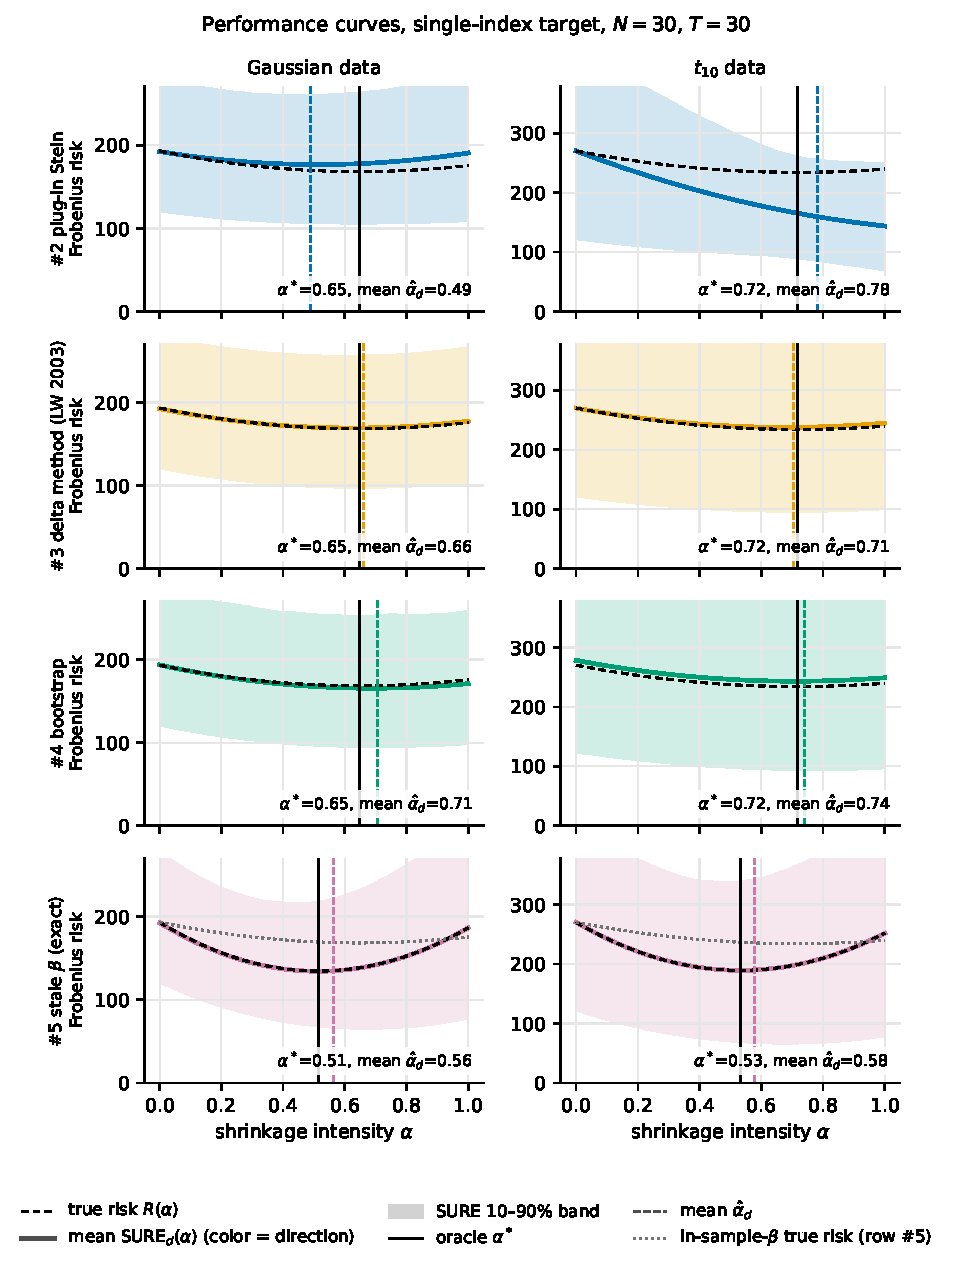
\includegraphics[width=5.6in]{si_curves.pdf}
\caption{Performance curves at $N = 30$, $T = 30$. Rows: directions \#2--\#5. Columns: Gaussian and $t_{10}$ data. Dashed black: true risk. Solid colored: mean $\mathrm{SURE}_d(\alpha)$, with its $10$--$90\%$ band across replications (clipped at the top of the panel). Solid vertical: $\alpha^*$. Dashed vertical: mean $\hat\alpha_d$. In row \#5 the true curve is that of the stale-beta estimator, and the dotted gray curve is the in-sample-beta true risk, for comparison.}\label{fig:curves}
\end{figure}

\begin{figure}[t]
\centering
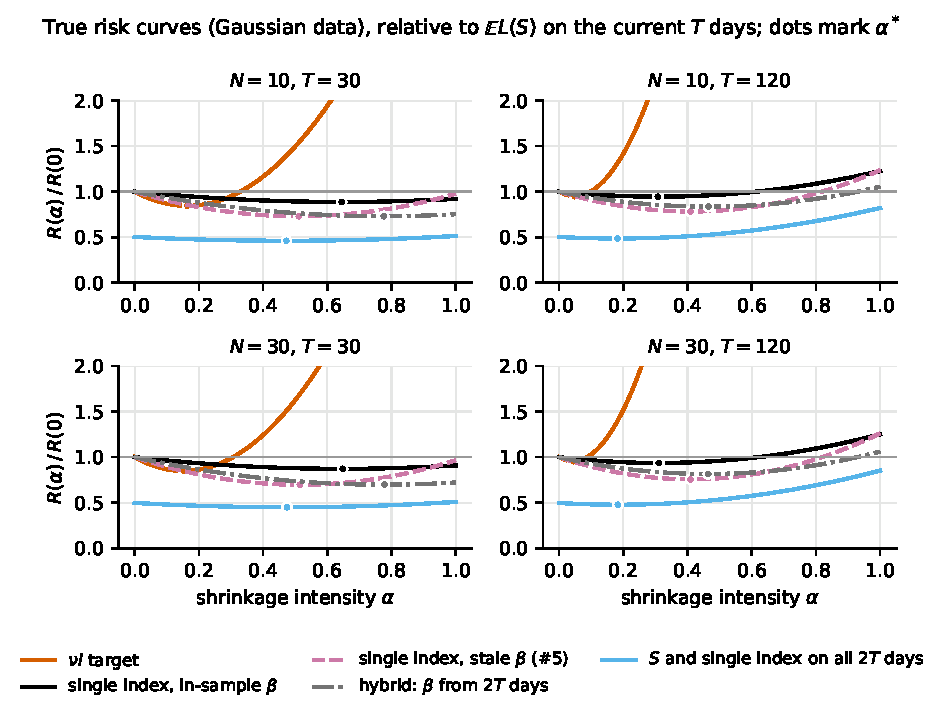
\includegraphics[width=6in]{si_targets.pdf}
\caption{True risk curves on the same Gaussian factor data, relative to $\mathbb{E}L(S)$ for $S$ on the current $T$ days: $\nu I$, single index with in-sample betas, single index with stale betas (\#5), the hybrid target (betas from all $2T$ days), and the single-index estimator computed entirely on all $2T$ days (its value at $\alpha = 0$ is the pooled $S$). Dots mark each curve's $\alpha^*$.}\label{fig:targets}
\end{figure}

\begin{figure}[t]
\centering
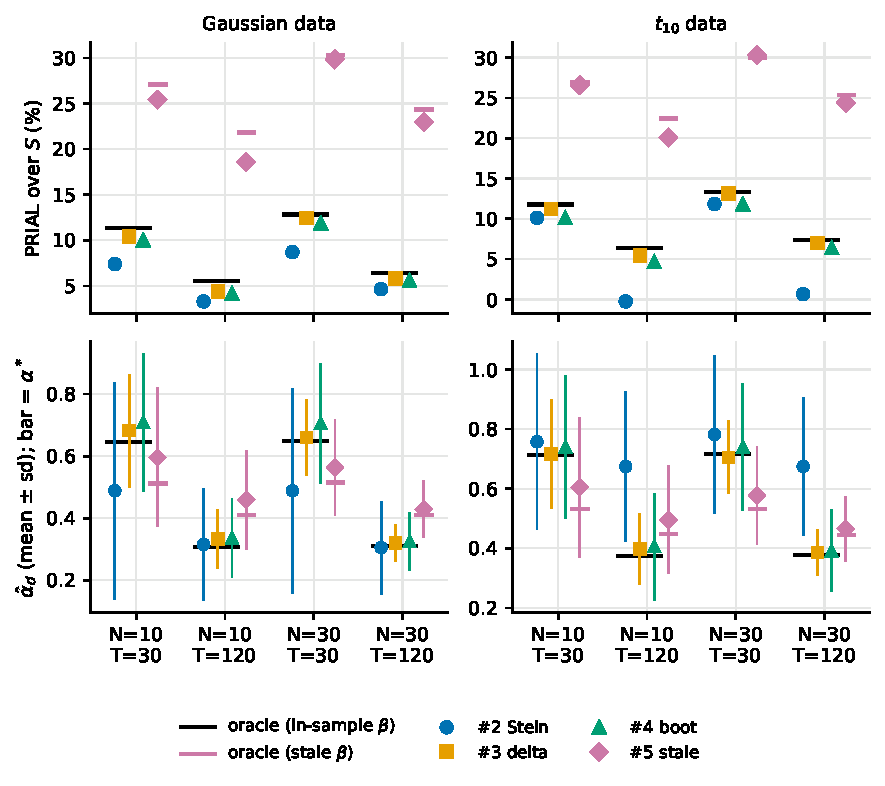
\includegraphics[width=6in]{si_prial.pdf}
\caption{Top: PRIAL of each direction's $\hat\alpha_d$. Horizontal bars show the oracle PRIAL, black for the in-sample target (\#2--\#4) and pink for the stale target (\#5). Bottom: mean $\pm$ sd of $\hat\alpha_d$; bars mark $\alpha^*$.}\label{fig:prial}
\end{figure}

\begin{table}[t]
\centering
\small
\caption{Bias ratio $\mathbb{E}\hat C^{(d)}_{\mathrm{off}}/C_{\mathrm{off}}$ (1 = unbiased; the Monte Carlo truth has a standard error of $1.7$--$2.9\%$ for the in-sample $C_{\mathrm{off}}$ and $3.4$--$5.8\%$ for the stale one) and PRIAL (\%). ``Oracle'' is the PRIAL at $\alpha^*$ of the in-sample target (for \#2--\#4) or of the stale target (for \#5). Full output, including $z$-scores, is in \texttt{sims/out/si\_results.txt}.}\label{tab:results}
\begin{tabular}{@{}llr|rrrr|rrrr|rr@{}}
\toprule
 & & & \multicolumn{4}{c|}{bias ratio} & \multicolumn{4}{c|}{PRIAL, in-sample target} & \multicolumn{2}{c}{PRIAL, stale} \\
data & $N$ & $T$ & \#2 & \#3 & \#4 & \#5 & \#2 & \#3 & \#4 & oracle & \#5 & oracle \\
\midrule
Gaussian & 10 & 30  & 1.06 & 1.02 & 0.99 & 1.02 & 7.4 & 10.4 & 10.0 & 11.4 & 25.4 & 27.1 \\
         & 10 & 120 & 0.96 & 0.95 & 0.95 & 0.90 & 3.3 & 4.4 & 4.1 & 5.6 & 18.6 & 21.8 \\
         & 30 & 30  & 1.05 & 1.00 & 0.98 & 0.99 & 8.7 & 12.4 & 11.9 & 12.8 & 29.8 & 30.3 \\
         & 30 & 120 & 1.00 & 0.99 & 0.98 & 0.97 & 4.6 & 5.8 & 5.6 & 6.4 & 23.0 & 24.3 \\
\midrule
$t_{10}$ & 10 & 30  & 0.77 & 1.01 & 1.00 & 1.00 & 10.1 & 11.2 & 10.1 & 11.8 & 26.6 & 27.0 \\
         & 10 & 120 & 0.70 & 0.97 & 0.99 & 0.95 & $-0.3$ & 5.5 & 4.6 & 6.3 & 20.1 & 22.4 \\
         & 30 & 30  & 0.77 & 1.01 & 1.04 & 1.00 & 11.8 & 13.1 & 11.8 & 13.3 & 30.3 & 29.9 \\
         & 30 & 120 & 0.75 & 1.03 & 1.04 & 1.06 & 0.6 & 7.0 & 6.4 & 7.4 & 24.4 & 25.4 \\
\bottomrule
\end{tabular}
\end{table}

\paragraph{The cross-term estimates.}
\begin{itemize}
  \item \emph{\#3 (delta method) is the best of the in-sample directions.} Its bias ratio is within $0.95$--$1.03$ in every cell, and the paired $z$-score of $\hat C^{(3)}_{\mathrm{off}} - C_{\mathrm{off}}$ satisfies $|z| \le 1.85$ everywhere, so no bias is detectable at this precision. Its mean SURE curve lies on the true curve (largest gap $2.7\%$ of $R(0)$ over all cells and $\alpha$), and its $\hat\alpha$ has the smallest spread of any direction. It reaches $91$--$99\%$ of the oracle PRIAL in the $N = 30$ cells and $79$--$95\%$ in the $N = 10$ cells. It does this under both Gaussian and $t_{10}$ data.
  \item \emph{\#4 (bootstrap)} is about as unbiased as \#3 (ratios $0.95$--$1.04$; paired $|z| \le 0.9$ except $t_{10}$, $N = 10$, $T = 120$, where $z = -3.6$ on its $2{,}000$-replication subset), but its $\hat\alpha$ is noisier (sd $0.09$--$0.24$ against $0.06$--$0.18$), because of the finite $B$ and the extra nonlinear terms. It always gets a slightly lower PRIAL than \#3, and costs about $200$ times more computation.\footnote{The PRIAL of \#4, and its gap to the oracle, are computed on the $2{,}000$-replication bootstrap subset; on that subset the oracle PRIAL is slightly different (e.g.\ $11.3$ against the table's $11.4$ for Gaussian, $N = 10$, $T = 30$).}
  \item \emph{\#2 (plug-in Stein)} is roughly unbiased under Gaussian data ($0.96$--$1.06$; the upward bias at $T = 30$ is detectable, $z = +4.3$ and $+3.2$, and vanishes at $T = 120$) but has a very noisy $\hat\alpha$ (sd up to $0.35$, with $26$--$32\%$ of the $T = 30$ draws clipped), so its PRIAL is only $59$--$72\%$ of the oracle. Under $t_{10}$ data it underestimates $C_{\mathrm{off}}$ by $23$--$30\%$ ($z$ between $-14.3$ and $-9.7$), because it imposes Gaussian fourth moments. That inflates $\hat\alpha$ (mean $0.67$ against $\alpha^* = 0.38$ at $T = 120$), and its PRIAL falls to about zero. At $T = 30$ it does better under $t_{10}$ ($86$--$89\%$ of the oracle), because there $\alpha^*$ is large and clipping $\hat\alpha$ at $1$ limits the damage. Figure~\ref{fig:curves} (top right) shows the mean SURE curve well below the true one.
  \item \emph{\#5 (stale betas)} is exactly unbiased, as Theorem~\ref{thm:stale} says. Its mean SURE curve is indistinguishable from $\tilde R$ (Figure~\ref{fig:curves}, bottom row), and it reaches $85$--$101\%$ of its own oracle PRIAL. A data-driven $\hat\alpha$ can beat the fixed $\tilde\alpha^*$ slightly, because it adapts to each sample. The table ratios that differ from $1$ (e.g.\ $0.90$) are Monte Carlo noise in the truth: the paired $z$ is $-1.9$, and the high-replication check (c) gives $1.001$.
\end{itemize}

\paragraph{Why the stale target looks better, and why that is not a free lunch.}
At first sight the stale-beta estimator is far better than the in-sample one: its oracle PRIAL is $22$--$30\%$, against $6$--$13\%$ (Figures~\ref{fig:targets}--\ref{fig:prial}). The comparison is not fair, because \#5 uses $T_0 = T$ extra days. Table~\ref{tab:bench} puts the extra days to other uses. Under stationarity, simply pooling all $2T$ days into one $S$, with no shrinkage at all, gives a PRIAL of about $50\%$, and running the in-sample single-index estimator on all $2T$ days gives $51$--$55\%$. Both dominate \#5 in every cell. The hybrid, which takes the betas from all $2T$ days but keeps $S$ and $s_{00}^2$ from the current window, is no better than \#5 (equal within $0.3$ points, or worse by up to $6$ points at $T = 120$). Using the extra days only for the betas wastes most of them. Splitting a \emph{fixed} window instead (betas from the first half, $S$ from the second half) is disastrous: PRIAL $-39$ to $-48\%$, because $S$ on $T/2$ days has about twice the risk of $S$ on $T$ days. So, under stationarity, (A1) together with (A7), \#5 is dominated by pooling.

\begin{table}[t]
\centering
\small
\caption{Oracle PRIAL (\%) against $\mathbb{E}L(S)$ for $S$ on the current $T$ days, by how the data are used. ``Pooled $S$'' uses no shrinkage. ``Split'' uses only the current $T$ days (Gaussian only). $20{,}000$ replications ($10{,}000$ for split).}\label{tab:bench}
\begin{tabular}{@{}llr|rr|rrrr|r@{}}
\toprule
 & & & \multicolumn{2}{c|}{current $T$ days only} & \multicolumn{4}{c|}{uses $T_0 = T$ earlier days} & \\
data & $N$ & $T$ & $\nu I$ & in-sample SI & \#5 stale & hybrid & pooled $S$ & pooled SI & split \\
\midrule
Gaussian & 10 & 30  & 15.6 & 11.4 & 27.1 & 27.0 & 49.7 & 54.0 & $-44.5$ \\
         & 10 & 120 & 4.8 & 5.6 & 21.8 & 16.5 & 49.8 & 51.5 & $-48.4$ \\
         & 30 & 30  & 15.1 & 12.8 & 30.3 & 30.3 & 50.2 & 55.0 & $-39.4$ \\
         & 30 & 120 & 4.3 & 6.4 & 24.3 & 18.5 & 50.3 & 52.2 & $-43.0$ \\
\midrule
$t_{10}$ & 10 & 30  & 20.4 & 11.8 & 27.0 & 27.0 & 50.0 & 54.6 & --- \\
         & 10 & 120 & 6.2 & 6.3 & 22.4 & 17.9 & 50.5 & 52.5 & --- \\
         & 30 & 30  & 19.7 & 13.3 & 29.9 & 30.2 & 49.8 & 55.1 & --- \\
         & 30 & 120 & 5.5 & 7.4 & 25.4 & 20.4 & 49.9 & 52.1 & --- \\
\bottomrule
\end{tabular}
\end{table}

Why does \#5 still beat the in-sample target on the same $T$ days? The two targets are about equally good on their own (at $\alpha = 1$ the curves nearly meet); the difference is their correlation with $S$. The in-sample $C_{\mathrm{off}}$ is about twice the stale one, and a target correlated with $S$ averages away less of the noise of $S$. An exact identity shows where this comes from. Let $b_i = \sigma_{0i}/\sigma_m^2$ be the population regression slopes and $e_{ti} = x_{ti} - b_im_t$. No independence is assumed; $\mathbb{E}[m_te_{ti}] = 0$ holds by construction. Write $u_i = \frac{1}{T}\sum_t m_te_{ti}$, $s^e_{ij} = \frac{1}{T}\sum_t e_{ti}e_{tj}$ and $B = s_{00}^2$. Then, for $i \ne j$,
\begin{align*}
  s_{ij} &= b_ib_jB + b_iu_j + b_ju_i + s^e_{ij}, \\
  f_{ij} &= b_ib_jB + b_iu_j + b_ju_i + u_iu_j/B, \\
  \tilde f_{ij} &= B\,\tilde\beta_i\tilde\beta_j .
\end{align*}
So $f_{ij} - s_{ij} = u_iu_j/B - s^e_{ij}$. The in-sample target contains the same beta-estimation noise $b_iu_j + b_ju_i$ as $S$, and shrinking toward it cannot remove that noise; only the residual part $s^e_{ij}$ is averaged away. The stale target does not contain $u$, so shrinking toward it averages away the $u$ terms too, at the price of independent stale-beta noise. Both targets keep the market-variance noise $b_ib_j(B - \sigma_m^2)$.

\begin{figure}[t]
\centering
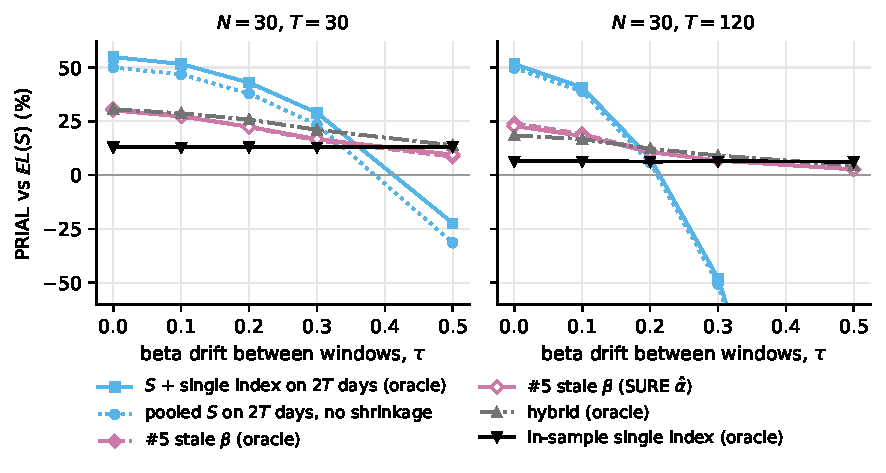
\includegraphics[width=6in]{si_drift.pdf}
\caption{Drifting betas ($N = 30$, Gaussian): the earlier window has betas $b + \tau\xi$. PRIAL against $\mathbb{E}L(S)$ on the current $T$ days. The pooled curves fall below the panel at large $\tau$ (to about $-250\%$ at $T = 120$, $\tau = 0.5$).}\label{fig:drift}
\end{figure}

\paragraph{Drifting betas.}
The only case for \#5 is non-stationarity: pooling assumes the earlier days have the same $\Sigma$, while Theorem~\ref{thm:stale} only needs them to be independent. Figure~\ref{fig:drift} lets the betas drift between windows by $\tau$ per asset (the betas range over $[0.5, 1.5]$). Pooling degrades fast. At $T = 30$ it still beats \#5 up to $\tau = 0.3$ (pooled single index $28.9$ against $16.7$) and loses at $\tau = 0.5$ ($-22.3$ against $9.5$). At $T = 120$ the crossover is near $\tau = 0.2$ ($7.9$ against $10.7$), and at $\tau = 0.5$ pooling has PRIAL $-241\%$. Throughout, the SURE of \#5 stays exactly unbiased (all ten bias $z$-scores within $\pm2.3$), and its data-driven $\hat\alpha$ stays within about $1.4$ points of its own oracle. However, \#5 is never the best option in this experiment. Wherever it beats pooling, the hybrid ($25.8$, $21.1$, $13.8$ at $T = 30$; $12.3$, $9.1$, $4.5$ at $T = 120$, for $\tau \ge 0.2$) or the in-sample single index (about $13$ and $6.4$) does at least as well. And at large drift, \#5 falls below the in-sample single index that uses no extra data at all. The hybrid has no exact SURE, though. The honest conclusion is that \#5's distinctive property is an exactly unbiased risk curve that remains valid when the windows differ, not a lower risk.

\paragraph{The $\nu I$ target is competitive with the in-sample single index at small $T$.}
Contrary to the motivating expectation, the in-sample single-index curve does not dip much lower than the $\nu I$ curve. Under Gaussian data at $T = 30$ the $\nu I$ oracle PRIAL is higher: $15.6$ against $11.4$ ($N = 10$) and $15.1$ against $12.8$ ($N = 30$). At $T = 120$ the single index is better: $5.6$ against $4.8$ and $6.4$ against $4.3$. The $\nu I$ optimum sits at a small $\alpha$ ($0.04$--$0.16$ under Gaussian data). Under $t_{10}$ data $\nu I$ wins by more at $T = 30$ ($20.4$ against $11.8$, and $19.7$ against $13.3$) and ties or loses at $T = 120$ ($6.2$ against $6.3$, and $5.5$ against $7.4$).

The design sensitivity check ($N = 30$, Gaussian) shows what drives this. The driver is misspecification. With no second factor ($g = 0$) the single index wins clearly: $16.5$ against $13.4$ at $T = 30$, and $16.9$ against $3.8$ at $T = 120$, with $\alpha^* \approx 1$. A stronger market does \emph{not} help the single index. With $\sigma_m^2 = 4$ it does worse: $1.7$ against $7.3$ for $\nu I$ at $T = 30$, and $0.8$ against $1.9$ at $T = 120$. The identity above explains why: the market-variance noise $b_ib_j(B - \sigma_m^2)$ appears in both $S$ and $F$, so shrinking toward $F$ cannot reduce it, and its variance grows like $\sigma_m^4$. The $\nu I$ target sets the off-diagonal entries to zero, which removes that noise (at the price of bias).

\section{Summary}

\begin{table}[h]
\centering
\small
\begin{tabular}{@{}>{\raggedright\arraybackslash}p{2.6cm}>{\raggedright\arraybackslash}p{2.9cm}>{\raggedright\arraybackslash}p{3.4cm}>{\raggedright\arraybackslash}p{6.1cm}@{}}
\toprule
Direction & Assumptions & Exact? & Performance (this simulation) \\
\midrule
\#2 plug-in Stein & A1--A5 (normality) & No: plug-in bias $O(1/T)$; wrong under non-normal tails & Bias ratio $0.96$--$1.06$ (Gaussian), $0.70$--$0.77$ ($t_{10}$); noisiest $\hat\alpha$; PRIAL $59$--$72\%$ of oracle (Gaussian), $\approx 0$ ($t_{10}$, $T = 120$). \\
\#3 delta method (LW 2003) & A1--A4 (+A6, A8 for accuracy) & No: first order, exact as $T \to \infty$ & Ratio $0.95$--$1.03$; mean SURE on the true curve; $79$--$99\%$ of oracle PRIAL; best in-sample direction, cheap. \\
\#4 bootstrap & A1--A4 (+A6, A8) & No: empirical-distribution covariance & Ratio $0.95$--$1.04$; noisier $\hat\alpha$ than \#3; slightly lower PRIAL; $\sim$200$\times$ the cost. \\
\#5 stale $\beta$ & A1--A4, A7 & Yes, exactly unbiased and distribution-free (Theorem~\ref{thm:stale}) & Verified unbiased ($|z| \le 1.02$); $85$--$101\%$ of its own oracle. Under stationarity it is dominated by pooling the $T_0$ extra days ($\approx 50\%$ PRIAL with no shrinkage, $51$--$55\%$ with the pooled single index, against $22$--$30\%$). Under drifting betas it beats pooling, and its SURE stays exactly unbiased, but the hybrid or the in-sample single index does at least as well. \\
\#1 condition on market & to be developed & --- & --- \\
\bottomrule
\end{tabular}
\end{table}

\paragraph{Open questions.}
\begin{enumerate}
  \item \emph{Resolved:} the stale-beta gain is an artifact of extra data. Pooling the $T_0$ days dominates \#5 under stationarity, and splitting a fixed window is disastrous (Table~\ref{tab:bench}). There is no free lunch.
  \item Under drift (Figure~\ref{fig:drift}), can an exactly unbiased SURE be built for the hybrid or for a down-weighted pooled estimator, which do better than \#5 there? The drift model here (independent drift per asset, constant within a window) is also only one choice.
  \item Can a bias correction make \#3 exactly unbiased, for instance with U-statistic versions of the products in the gradient, in the way Section~5 replaced $\operatorname{tr}(S^2)$ by $\hat U_2$?
  \item The single index beats $\nu I$ clearly only when the single-index model is (nearly) correct ($g = 0$); a stronger market makes it worse. Which regime describes real returns, where industry factors are present, decides whether the single-index target is worth its cost.
\end{enumerate}

\bibliographystyle{apalike}
\bibliography{refs}
\end{document}
